\documentclass[11pt,a4paper]{article}

% ── Packages ──────────────────────────────────────────────────────────────────
\usepackage[margin=1in]{geometry}
\usepackage{graphicx}
\usepackage{tikz}
\usetikzlibrary{shapes.geometric, arrows.meta, positioning, fit, calc, decorations.pathreplacing}
\usepackage{xcolor}
\usepackage{hyperref}
\usepackage{listings}
\usepackage{booktabs}
\usepackage{enumitem}
\usepackage{fancyhdr}
\usepackage{tcolorbox}
\usepackage{multicol}
\usepackage{tabularx}
\usepackage{float}
\usepackage{caption}
\usepackage{parskip}

% ── Colors ────────────────────────────────────────────────────────────────────
\definecolor{gold}{HTML}{D4A843}
\definecolor{darkbg}{HTML}{080706}
\definecolor{reactblue}{HTML}{61DAFB}
\definecolor{nodegreen}{HTML}{68A063}
\definecolor{pythonyellow}{HTML}{FFD43B}
\definecolor{claudepurple}{HTML}{7C3AED}
\definecolor{codebg}{HTML}{1E1E2E}
\definecolor{softgray}{HTML}{F5F5F5}
\definecolor{linkblue}{HTML}{2563EB}

% ── Hyperref config ──────────────────────────────────────────────────────────
\hypersetup{
    colorlinks=true,
    linkcolor=linkblue,
    urlcolor=linkblue,
    citecolor=linkblue,
    pdftitle={TripMind Architecture},
    pdfauthor={TripMind Team},
}

% ── Code listing style ───────────────────────────────────────────────────────
\lstset{
    basicstyle=\ttfamily\small,
    backgroundcolor=\color{softgray},
    frame=single,
    rulecolor=\color{gray!40},
    breaklines=true,
    breakatwhitespace=true,
    tabsize=2,
    showstringspaces=false,
    numbers=left,
    numberstyle=\tiny\color{gray},
    keywordstyle=\color{claudepurple}\bfseries,
    stringstyle=\color{nodegreen},
    commentstyle=\color{gray}\itshape,
}

% ── Header / Footer ─────────────────────────────────────────────────────────
\pagestyle{fancy}
\fancyhf{}
\fancyhead[L]{\textsc{TripMind Architecture}}
\fancyhead[R]{\textsc{v3.0}}
\fancyfoot[C]{\thepage}
\renewcommand{\headrulewidth}{0.4pt}

% ── Custom tcolorbox styles ──────────────────────────────────────────────────
\newtcolorbox{infobox}[1][]{
    colback=softgray,
    colframe=gold,
    fonttitle=\bfseries,
    title=#1,
    arc=2mm,
    boxrule=0.8pt,
}

\newtcolorbox{techbox}[1][]{
    colback=white,
    colframe=claudepurple!70,
    fonttitle=\bfseries,
    title=#1,
    arc=2mm,
    boxrule=0.6pt,
}

% ══════════════════════════════════════════════════════════════════════════════
\begin{document}

% ── Title Page ───────────────────────────────────────────────────────────────
\begin{titlepage}
\centering
\vspace*{3cm}

{\Huge\bfseries TripMind}\\[0.5cm]
{\Large AI Travel Planner with Real-Time Verification}\\[2cm]

{\large\textsc{System Architecture Document}}\\[0.5cm]
{\large Version 3.0}\\[3cm]

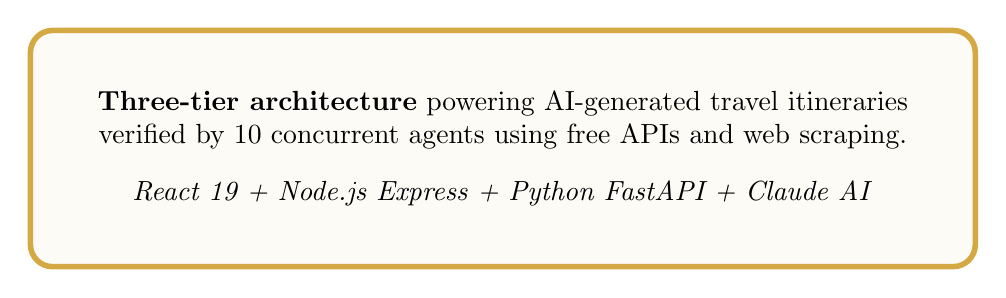
\begin{tikzpicture}
    \node[draw=gold, line width=2pt, rounded corners=8pt, minimum width=12cm, minimum height=3cm, fill=gold!5] {
        \begin{minipage}{11cm}
        \centering
        \textbf{Three-tier architecture} powering AI-generated travel itineraries\\
        verified by 10 concurrent agents using free APIs and web scraping.\\[0.3cm]
        \textit{React 19 + Node.js Express + Python FastAPI + Claude AI}
        \end{minipage}
    };
\end{tikzpicture}

\vfill
{\small Last updated: March 2026}
\end{titlepage}

% ── Table of Contents ────────────────────────────────────────────────────────
\tableofcontents
\newpage

% ══════════════════════════════════════════════════════════════════════════════
\section{System Overview}
% ══════════════════════════════════════════════════════════════════════════════

TripMind is an AI-powered travel planning application that generates personalized trip itineraries and then independently verifies every detail---hotel prices, flight costs, weather forecasts, safety advisories, place existence, reviews, and more---through 10 concurrent verification agents.

\begin{infobox}[Key Design Principles]
\begin{itemize}[nosep]
    \item \textbf{Split-prompt strategy:} Two Claude API calls (skeleton + days) to avoid token truncation on long trips.
    \item \textbf{SSE streaming:} Both trip generation and verification stream results to the browser in real time.
    \item \textbf{Fan-out/fan-in concurrency:} All 10 agents run in parallel via \texttt{asyncio.gather()}.
    \item \textbf{Graceful degradation:} The app works fully without the Python service (shows AI estimates).
    \item \textbf{Zero cost APIs:} All verification uses free APIs and web scraping---only the Claude API has a cost.
    \item \textbf{Fallback chains:} Scraping agents never fully fail; each has 2--3 fallback data sources.
\end{itemize}
\end{infobox}

% ── High-Level Architecture Diagram ──────────────────────────────────────────
\subsection{High-Level Architecture}

\begin{figure}[H]
\centering
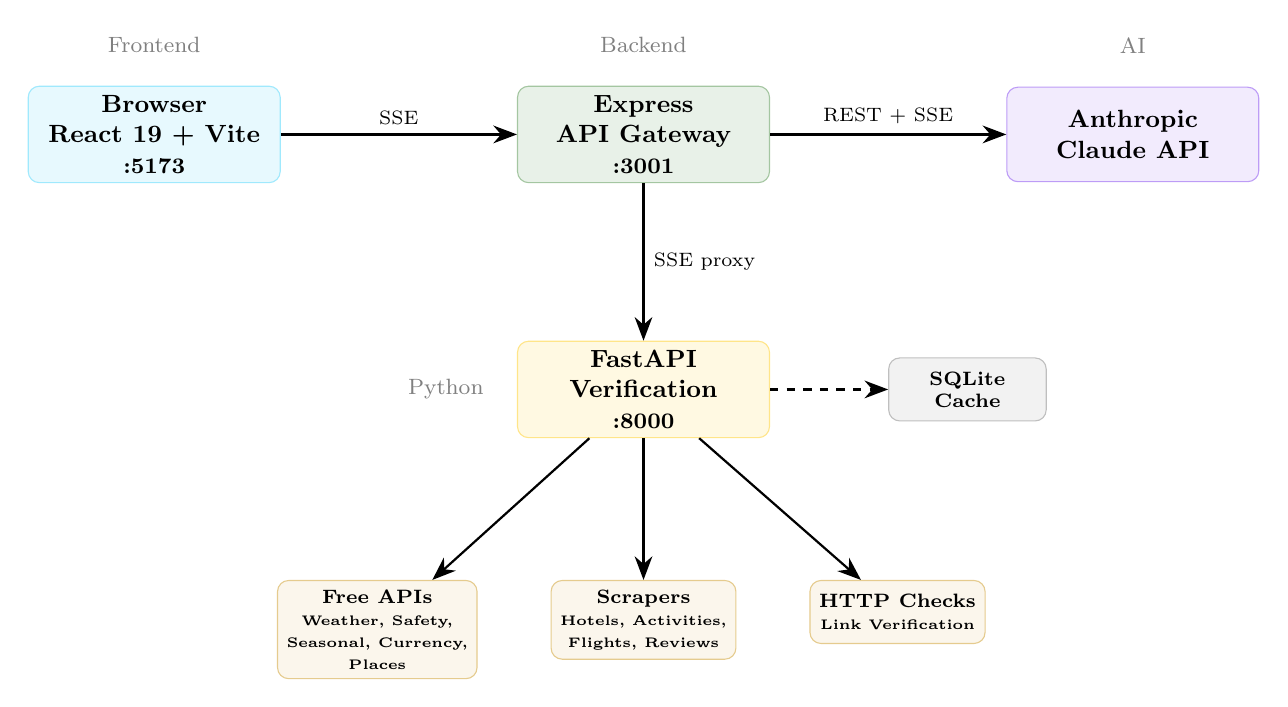
\begin{tikzpicture}[
    node distance=1.5cm and 2.5cm,
    box/.style={draw, rounded corners=4pt, minimum width=3.2cm, minimum height=1.2cm, align=center, font=\small\bfseries},
    svc/.style={box, fill=nodegreen!15, draw=nodegreen!60},
    ext/.style={box, fill=claudepurple!10, draw=claudepurple!50},
    ui/.style={box, fill=reactblue!15, draw=reactblue!60},
    py/.style={box, fill=pythonyellow!15, draw=pythonyellow!60},
    arr/.style={-{Stealth[length=3mm]}, thick},
    darr/.style={-{Stealth[length=3mm]}, thick, dashed},
]

% Nodes
\node[ui] (browser) {Browser\\React 19 + Vite\\{\footnotesize :5173}};
\node[svc, right=3cm of browser] (express) {Express\\API Gateway\\{\footnotesize :3001}};
\node[ext, right=3cm of express] (claude) {Anthropic\\Claude API};
\node[py, below=2cm of express] (fastapi) {FastAPI\\Verification\\{\footnotesize :8000}};

% Agent fan-out
\node[box, fill=gold!10, draw=gold!60, below left=1.8cm and 0.5cm of fastapi, minimum width=2.2cm, minimum height=0.8cm, font=\scriptsize\bfseries] (a1) {Free APIs\\{\tiny Weather, Safety,}\\{\tiny Seasonal, Currency,}\\{\tiny Places}};
\node[box, fill=gold!10, draw=gold!60, below=1.8cm of fastapi, minimum width=2.2cm, minimum height=0.8cm, font=\scriptsize\bfseries] (a2) {Scrapers\\{\tiny Hotels, Activities,}\\{\tiny Flights, Reviews}};
\node[box, fill=gold!10, draw=gold!60, below right=1.8cm and 0.5cm of fastapi, minimum width=2.2cm, minimum height=0.8cm, font=\scriptsize\bfseries] (a3) {HTTP Checks\\{\tiny Link Verification}};

% SQLite
\node[box, fill=gray!10, draw=gray!50, right=1.5cm of fastapi, minimum width=2cm, minimum height=0.8cm, font=\scriptsize\bfseries] (cache) {SQLite\\Cache};

% Arrows
\draw[arr] (browser) -- node[above, font=\scriptsize] {SSE} (express);
\draw[arr] (express) -- node[above, font=\scriptsize] {REST + SSE} (claude);
\draw[arr] (express) -- node[right, font=\scriptsize] {SSE proxy} (fastapi);
\draw[arr] (fastapi) -- (a1);
\draw[arr] (fastapi) -- (a2);
\draw[arr] (fastapi) -- (a3);
\draw[darr] (fastapi) -- (cache);

% Labels
\node[above=0.3cm of browser, font=\footnotesize\color{gray}] {Frontend};
\node[above=0.3cm of express, font=\footnotesize\color{gray}] {Backend};
\node[above=0.3cm of claude, font=\footnotesize\color{gray}] {AI};
\node[left=0.3cm of fastapi, font=\footnotesize\color{gray}] {Python};

\end{tikzpicture}
\caption{High-level system architecture showing the three services and their connections.}
\label{fig:architecture}
\end{figure}

% ── Technology Stack ─────────────────────────────────────────────────────────
\subsection{Technology Stack}

\begin{table}[H]
\centering
\begin{tabularx}{\textwidth}{l l X}
\toprule
\textbf{Layer} & \textbf{Technology} & \textbf{Purpose} \\
\midrule
Frontend & React 19 + Vite & Component-based UI with HMR \\
Styling & CSS Modules & Scoped styles with design tokens \\
State & React Context & Form state, trip data, verification \\
Backend & Node.js + Express & API gateway, rate limiting, SSE proxy \\
AI & Anthropic Claude API & Trip itinerary generation (streaming) \\
Verification & Python FastAPI & Agent orchestration, SSE streaming \\
Scraping & Playwright + httpx & Browser automation and HTTP scraping \\
Caching & SQLite (aiosqlite) & TTL-based result caching \\
PDF & @react-pdf/renderer & Client-side PDF generation (lazy-loaded) \\
\bottomrule
\end{tabularx}
\caption{Technology stack by layer.}
\end{table}


% ══════════════════════════════════════════════════════════════════════════════
\section{Frontend Architecture}
% ══════════════════════════════════════════════════════════════════════════════

% ── Component Tree ───────────────────────────────────────────────────────────
\subsection{Component Tree}

\begin{figure}[H]
\centering
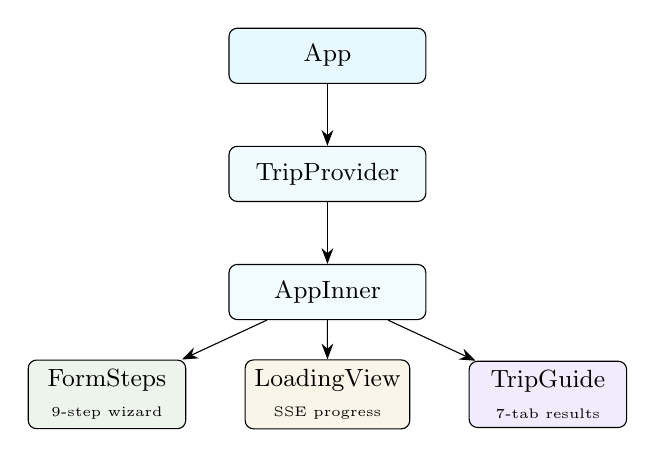
\begin{tikzpicture}[
    every node/.style={draw, rounded corners=3pt, minimum width=2.5cm, minimum height=0.7cm, font=\small, align=center},
    level 1/.style={sibling distance=5.5cm, level distance=1.5cm},
    level 2/.style={sibling distance=3.8cm, level distance=1.5cm},
    level 3/.style={sibling distance=2.8cm, level distance=1.3cm},
    edge from parent/.style={draw, -{Stealth[length=2mm]}},
]

\node[fill=reactblue!15] {App}
    child { node[fill=reactblue!10] {TripProvider}
        child { node[fill=reactblue!8] {AppInner}
            child { node[fill=nodegreen!12, minimum width=2cm] {FormSteps\\{\tiny 9-step wizard}} }
            child { node[fill=gold!12, minimum width=2cm] {LoadingView\\{\tiny SSE progress}} }
            child { node[fill=claudepurple!10, minimum width=2cm] {TripGuide\\{\tiny 7-tab results}} }
        }
    };

\end{tikzpicture}
\caption{React component tree. Only one of FormSteps/LoadingView/TripGuide renders at a time.}
\label{fig:component-tree}
\end{figure}

The application has three mutually exclusive view states:
\begin{enumerate}[nosep]
    \item \textbf{FormSteps} --- Shown when no trip is being generated and no results exist.
    \item \textbf{LoadingView} --- Shown during Claude API streaming (skeleton phase and days phase).
    \item \textbf{TripGuide} --- Shown when trip data is available, with verification running in the background.
\end{enumerate}

% ── Form Wizard ──────────────────────────────────────────────────────────────
\subsection{9-Step Form Wizard}

The form collects 24+ fields across 9 steps. Each step is a \texttt{switch} case in \texttt{FormSteps.jsx}:

\begin{figure}[H]
\centering
\begin{tikzpicture}[
    step/.style={draw, rounded corners=3pt, minimum width=1.8cm, minimum height=0.9cm, font=\scriptsize\bfseries, align=center},
    arr/.style={-{Stealth[length=2mm]}, thick, gold},
]

\foreach \i/\label/\fields [count=\n from 0] in {
    1/From/{origin, passport},
    2/To/{destinations},
    3/When/{dates, flexibility},
    4/Who/{adults, children,\\ group, occasions},
    5/Money/{budget, currency,\\ flexibility},
    6/Vibe/{trip types, activity\\ level, climate},
    7/Stay/{accommodation,\\ travel style},
    8/Details/{dietary, must-haves,\\ avoid, accessibility,\\ pet-friendly, workcation},
    9/Go/{review + generate}%
} {
    \node[step, fill=gold!8] (s\i) at (\n*1.65, 0) {\label};
    \node[font=\tiny, text width=1.6cm, align=center, below=0.15cm of s\i] {\fields};
}

\foreach \i [evaluate=\i as \j using int(\i+1)] in {1,...,8} {
    \draw[arr] (s\i) -- (s\j);
}

\end{tikzpicture}
\caption{Form wizard steps and the fields each step collects.}
\label{fig:form-steps}
\end{figure}

\begin{techbox}[Form Validation Rules]
\begin{itemize}[nosep]
    \item Step 1 (From): Requires non-empty \texttt{origin}.
    \item Step 3 (When): Requires both \texttt{dateFrom} and \texttt{dateTo}.
    \item Step 5 (Money): Requires non-empty \texttt{budget}.
    \item All other steps: freely passable (no required fields).
\end{itemize}
\end{techbox}


% ── State Management ─────────────────────────────────────────────────────────
\subsection{State Management}

All application state lives in a single React Context (\texttt{TripContext.jsx}):

\begin{table}[H]
\centering
\begin{tabularx}{\textwidth}{l l X}
\toprule
\textbf{State} & \textbf{Type} & \textbf{Purpose} \\
\midrule
\texttt{form} & Object (24+ fields) & All user inputs from the 9-step wizard \\
\texttt{step} & Integer (0--8) & Current wizard step \\
\texttt{loading} & Boolean & True during Claude API calls \\
\texttt{loadingPhase} & ``skeleton'' | ``days'' & Which generation phase is active \\
\texttt{streamText} & String & Accumulated streaming text (shown in LoadingView) \\
\texttt{tripData} & Object | null & Parsed trip plan (skeleton + days merged) \\
\texttt{verification} & Object | null & Verification results from all 10 agents \\
\texttt{verifying} & Boolean & True while agents are running \\
\texttt{error} & String | null & Error message for display \\
\bottomrule
\end{tabularx}
\caption{Key state variables in TripContext.}
\end{table}


% ══════════════════════════════════════════════════════════════════════════════
\section{Trip Generation Pipeline}
% ══════════════════════════════════════════════════════════════════════════════

Trip generation uses a two-phase ``split-prompt'' strategy to avoid token truncation on longer trips.

\subsection{Generation Flow}

\begin{figure}[H]
\centering
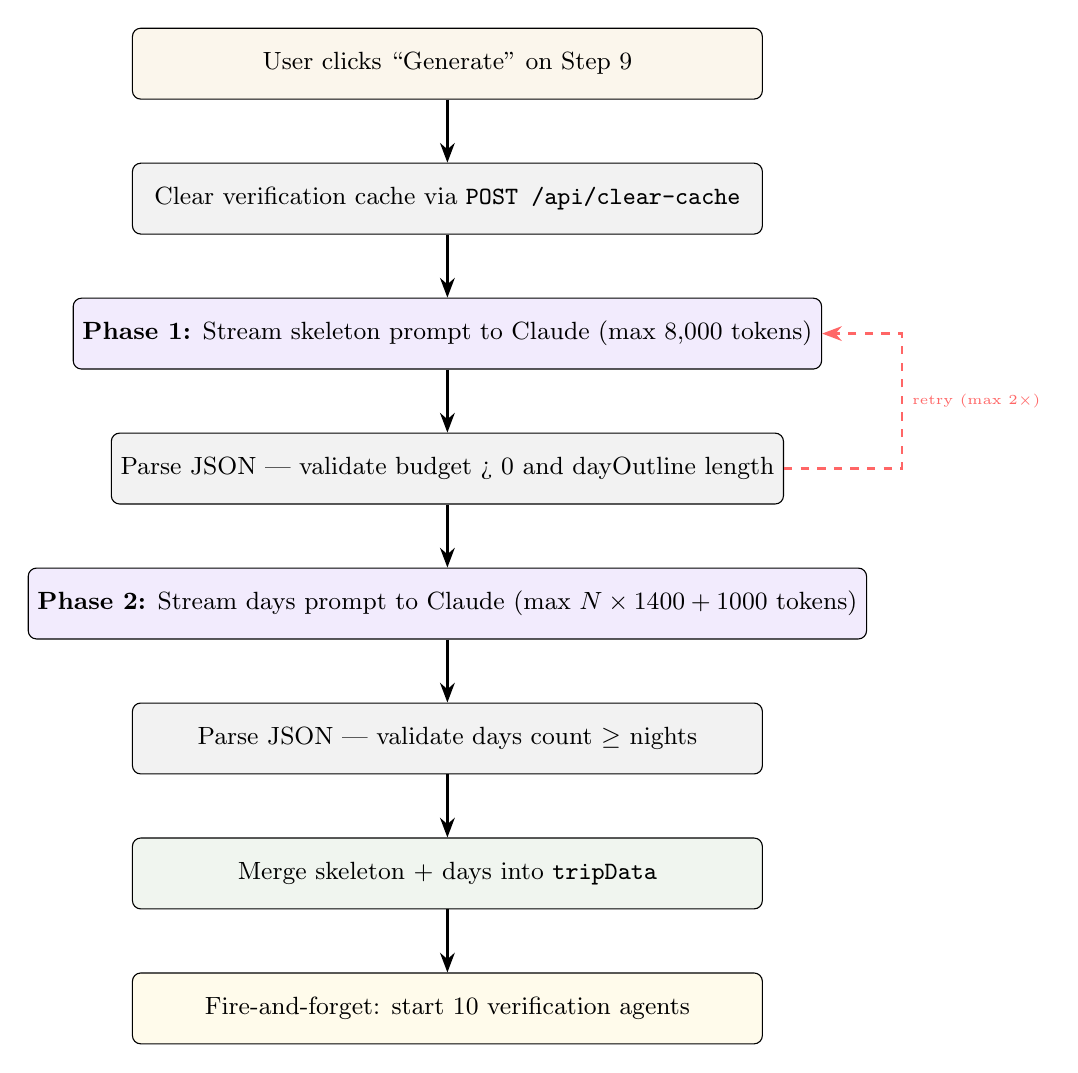
\begin{tikzpicture}[
    node distance=0.8cm,
    box/.style={draw, rounded corners=3pt, minimum width=8cm, minimum height=0.9cm, font=\small, align=center},
    arr/.style={-{Stealth[length=2.5mm]}, thick},
]

\node[box, fill=gold!10] (s1) {User clicks ``Generate'' on Step 9};
\node[box, fill=gray!10, below=of s1] (s2) {Clear verification cache via \texttt{POST /api/clear-cache}};
\node[box, fill=claudepurple!10, below=of s2] (s3) {\textbf{Phase 1:} Stream skeleton prompt to Claude (max 8,000 tokens)};
\node[box, fill=gray!10, below=of s3] (s4) {Parse JSON --- validate budget > 0 and dayOutline length};
\node[box, fill=claudepurple!10, below=of s4] (s5) {\textbf{Phase 2:} Stream days prompt to Claude (max $N \times 1400 + 1000$ tokens)};
\node[box, fill=gray!10, below=of s5] (s6) {Parse JSON --- validate days count $\geq$ nights};
\node[box, fill=nodegreen!10, below=of s6] (s7) {Merge skeleton + days into \texttt{tripData}};
\node[box, fill=pythonyellow!10, below=of s7] (s8) {Fire-and-forget: start 10 verification agents};

\foreach \a/\b in {s1/s2, s2/s3, s3/s4, s4/s5, s5/s6, s6/s7, s7/s8} {
    \draw[arr] (\a) -- (\b);
}

% Retry annotation
\draw[arr, dashed, red!60] (s4.east) -- ++(1.5,0) |- node[right, font=\tiny, pos=0.25] {retry (max 2$\times$)} (s3.east);

\end{tikzpicture}
\caption{Two-phase trip generation pipeline with retry logic.}
\label{fig:generation-flow}
\end{figure}


\subsection{Split-Prompt Strategy}

\begin{techbox}[Why Two Calls?]
A single Claude call for a 7-day trip with full activities, accommodations, flights, and budget would require 20,000+ tokens of output. At that length, the model often truncates the JSON mid-object, producing unparseable results. By splitting into skeleton (structure + budget + accommodations) and days (detailed activities), each call stays within a safe token budget.
\end{techbox}

\textbf{Phase 1 --- Skeleton Prompt} generates:
\begin{multicols}{2}
\begin{itemize}[nosep]
    \item Trip title, tagline, hero image keyword
    \item Budget breakdown by category
    \item Flight options with search queries
    \item Accommodation options per city
    \item Day outline (day number, date, location, theme)
    \item Insider tips, packing highlights
    \item Instagram accounts, YouTube searches
    \item Suggested splurges with booking keywords
\end{itemize}
\end{multicols}

\textbf{Phase 2 --- Days Prompt} receives the skeleton and generates:
\begin{itemize}[nosep]
    \item 3--4 activities per day with time, cost, Maps query, and booking keyword.
    \item One dining tip per day with Maps query.
    \item Image keywords for hero photos per day.
\end{itemize}

\subsection{JSON Recovery}

Claude occasionally produces malformed JSON (trailing commas, truncated output, unescaped characters). The \texttt{cleanAndParseJSON()} function applies a three-stage recovery:

\begin{enumerate}[nosep]
    \item Strip markdown code fences, find outermost \texttt{\{...\}}, remove trailing commas.
    \item On parse failure: escape unescaped newlines inside JSON strings.
    \item On second failure: repair truncated JSON---close open strings, remove partial key-value pairs, count unclosed braces/brackets with a state machine, and append closing characters.
\end{enumerate}


% ══════════════════════════════════════════════════════════════════════════════
\section{Backend (Express API Gateway)}
% ══════════════════════════════════════════════════════════════════════════════

The Express server on port 3001 serves as a Backend-for-Frontend (BFF), proxying requests to Claude and the Python verification service.

\subsection{Request Flow}

\begin{figure}[H]
\centering
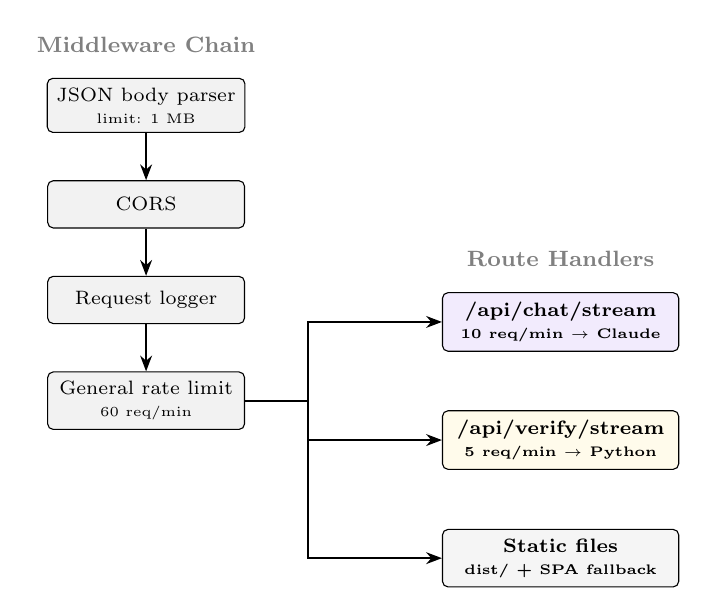
\begin{tikzpicture}[
    node distance=0.6cm and 2cm,
    mw/.style={draw, rounded corners=2pt, minimum width=2.5cm, minimum height=0.6cm, font=\scriptsize, align=center, fill=gray!10},
    route/.style={draw, rounded corners=2pt, minimum width=3cm, minimum height=0.6cm, font=\scriptsize\bfseries, align=center},
    arr/.style={-{Stealth[length=2mm]}, thick},
]

% Middleware chain
\node[mw] (m1) {JSON body parser\\{\tiny limit: 1 MB}};
\node[mw, below=of m1] (m2) {CORS};
\node[mw, below=of m2] (m3) {Request logger};
\node[mw, below=of m3] (m4) {General rate limit\\{\tiny 60 req/min}};

\foreach \a/\b in {m1/m2, m2/m3, m3/m4} {
    \draw[arr] (\a) -- (\b);
}

% Routes
\node[route, fill=claudepurple!10, right=2.5cm of m4, yshift=1cm] (r1) {/api/chat/stream\\{\tiny 10 req/min $\to$ Claude}};
\node[route, fill=pythonyellow!10, right=2.5cm of m4, yshift=-0.5cm] (r2) {/api/verify/stream\\{\tiny 5 req/min $\to$ Python}};
\node[route, fill=gray!8, right=2.5cm of m4, yshift=-2cm] (r3) {Static files\\{\tiny dist/ + SPA fallback}};

\draw[arr] (m4.east) -- ++(0.8,0) |- (r1.west);
\draw[arr] (m4.east) -- ++(0.8,0) |- (r2.west);
\draw[arr] (m4.east) -- ++(0.8,0) |- (r3.west);

\node[above=0.2cm of m1, font=\footnotesize\bfseries\color{gray}] {Middleware Chain};
\node[above=0.2cm of r1, font=\footnotesize\bfseries\color{gray}] {Route Handlers};

\end{tikzpicture}
\caption{Express middleware chain and route handlers.}
\label{fig:express}
\end{figure}

\subsection{SSE Streaming Proxy}

For Claude streaming (\texttt{/api/chat/stream}), the server:
\begin{enumerate}[nosep]
    \item Sets SSE headers: \texttt{Content-Type: text/event-stream}, \texttt{Cache-Control: no-cache}.
    \item Calls the Anthropic API with \texttt{stream: true}.
    \item Re-emits \texttt{content\_block\_delta} events as \texttt{data: \{"text": "..."\}}.
    \item Sends \texttt{data: [DONE]} on \texttt{message\_stop}.
\end{enumerate}

For verification streaming (\texttt{/api/verify/stream}), the server performs a raw byte pipe---forwarding SSE chunks from the Python service directly to the browser without parsing (120-second timeout).

\subsection{Rate Limits}

\begin{table}[H]
\centering
\begin{tabular}{l c c}
\toprule
\textbf{Route} & \textbf{Window} & \textbf{Max Requests} \\
\midrule
All \texttt{/api/*} routes & 60 seconds & 60 \\
\texttt{/api/chat}, \texttt{/api/chat/stream} & 60 seconds & 10 \\
\texttt{/api/verify}, \texttt{/api/verify/stream} & 60 seconds & 5 \\
\bottomrule
\end{tabular}
\caption{Express rate limiting configuration.}
\end{table}


% ══════════════════════════════════════════════════════════════════════════════
\section{Verification System}
% ══════════════════════════════════════════════════════════════════════════════

The verification system is a Python FastAPI microservice that runs 10 agents concurrently to cross-check every detail of the AI-generated trip plan against real-world data.

\subsection{Agent Orchestration}

\begin{figure}[H]
\centering
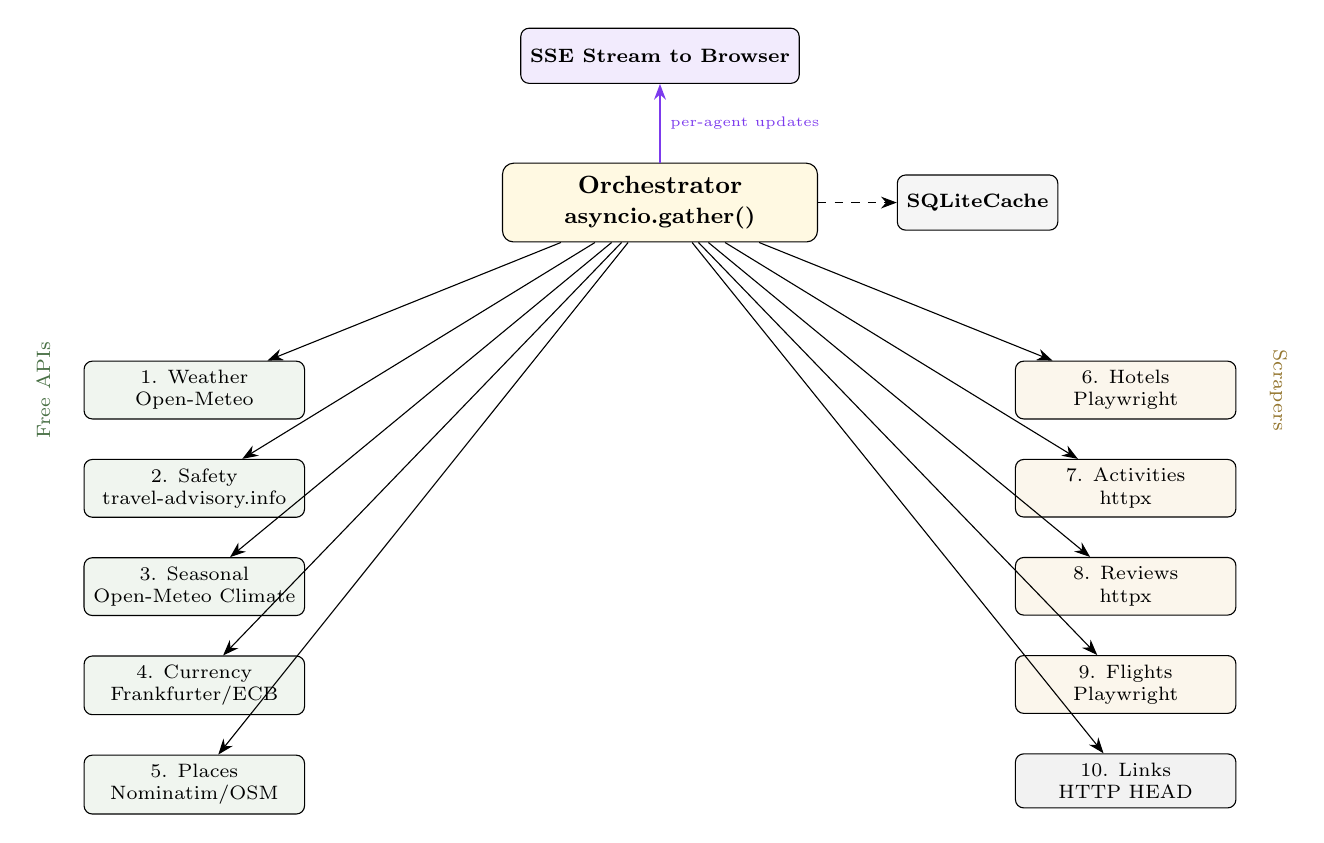
\begin{tikzpicture}[
    node distance=0.5cm,
    orch/.style={draw, rounded corners=4pt, minimum width=4cm, minimum height=1cm, font=\small\bfseries, align=center, fill=pythonyellow!15},
    agent/.style={draw, rounded corners=3pt, minimum width=2.8cm, minimum height=0.65cm, font=\scriptsize, align=center},
    free/.style={agent, fill=nodegreen!10},
    scrape/.style={agent, fill=gold!10},
    http/.style={agent, fill=gray!10},
    arr/.style={-{Stealth[length=2mm]}},
]

\node[orch] (orch) {Orchestrator\\{\footnotesize asyncio.gather()}};

% Fan out - left column (free APIs)
\node[free, below left=1.5cm and 2.5cm of orch] (w) {1. Weather\\Open-Meteo};
\node[free, below=of w] (sa) {2. Safety\\travel-advisory.info};
\node[free, below=of sa] (se) {3. Seasonal\\Open-Meteo Climate};
\node[free, below=of se] (cu) {4. Currency\\Frankfurter/ECB};
\node[free, below=of cu] (pl) {5. Places\\Nominatim/OSM};

% Right column (scrapers + http)
\node[scrape, below right=1.5cm and 2.5cm of orch] (ho) {6. Hotels\\Playwright};
\node[scrape, below=of ho] (ac) {7. Activities\\httpx};
\node[scrape, below=of ac] (re) {8. Reviews\\httpx};
\node[scrape, below=of re] (fl) {9. Flights\\Playwright};
\node[http, below=of fl] (li) {10. Links\\HTTP HEAD};

% Arrows from orchestrator
\foreach \n in {w, sa, se, cu, pl, ho, ac, re, fl, li} {
    \draw[arr] (orch) -- (\n);
}

% Cache on the side
\node[draw, rounded corners=3pt, fill=gray!8, minimum width=1.8cm, minimum height=0.7cm, font=\scriptsize\bfseries, right=1cm of orch] (cache) {SQLite\\Cache};
\draw[arr, dashed] (orch) -- (cache);

% Labels
\node[left=0.3cm of w, font=\scriptsize\color{nodegreen!70!black}, rotate=90, anchor=south] {Free APIs};
\node[right=0.3cm of ho, font=\scriptsize\color{gold!70!black}, rotate=270, anchor=south] {Scrapers};

% SSE output
\node[draw, rounded corners=3pt, fill=claudepurple!10, minimum width=3cm, minimum height=0.7cm, font=\scriptsize\bfseries, above=1cm of orch] (sse) {SSE Stream to Browser};
\draw[arr, thick, claudepurple] (orch) -- node[right, font=\tiny] {per-agent updates} (sse);

\end{tikzpicture}
\caption{Fan-out/fan-in agent orchestration. All 10 agents run in parallel via \texttt{asyncio.gather()}.}
\label{fig:orchestration}
\end{figure}


\subsection{Agent Details}

Each agent follows a consistent pattern:
\begin{enumerate}[nosep]
    \item Check if the agent is enabled in \texttt{config.py}.
    \item Build a cache key from the input parameters.
    \item Check \texttt{SQLite cache} for a valid (non-expired) result.
    \item On cache miss: call the underlying API or scraper.
    \item On success: store the result in cache with the agent's TTL.
    \item Return a Pydantic model (or \texttt{None} on failure).
\end{enumerate}

Each agent coroutine is wrapped in \texttt{asyncio.wait\_for(coro, timeout=45)} to prevent any single agent from blocking the pipeline.

\begin{table}[H]
\centering
\small
\begin{tabularx}{\textwidth}{c l l c X}
\toprule
\textbf{\#} & \textbf{Agent} & \textbf{Data Source} & \textbf{TTL} & \textbf{What It Verifies} \\
\midrule
1 & Weather & Open-Meteo API & 3h & Daily temp, rain, weather codes \\
2 & Safety & travel-advisory.info & 24h & Country risk score (0--5), advice \\
3 & Seasonal & Open-Meteo Climate & 7d & Monthly averages, tourism level \\
4 & Currency & Frankfurter (ECB) & 1h & Exchange rates vs.\ user's currency \\
5 & Places & Nominatim / OSM & 7d & Place existence, coordinates, address \\
6 & Hotels & Google Hotels + Booking & 6h & Real prices, ratings, booking URLs \\
7 & Activities & Viator + GetYourGuide & 12h & Activity prices, ratings, URLs \\
8 & Reviews & Google Search & 48h & Star ratings, review counts \\
9 & Flights & Google Flights & 1h & Prices, airlines, durations \\
10 & Links & HTTP HEAD & 24h & URL reachability \\
\bottomrule
\end{tabularx}
\caption{All 10 verification agents with their data sources and cache TTLs.}
\label{tab:agents}
\end{table}


\subsection{Fallback Chains}

Scraping agents are designed to never fully fail. Each has a chain of data sources:

\begin{figure}[H]
\centering
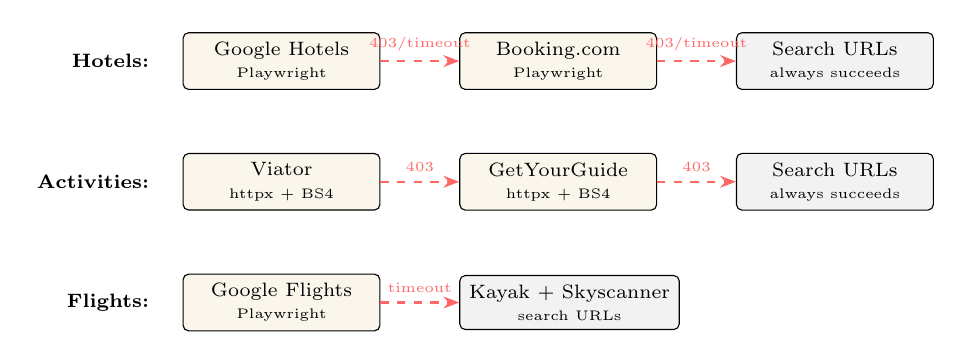
\begin{tikzpicture}[
    node distance=0.3cm and 1cm,
    src/.style={draw, rounded corners=2pt, minimum width=2.5cm, minimum height=0.6cm, font=\scriptsize, align=center},
    arr/.style={-{Stealth[length=2mm]}, thick},
    fail/.style={-{Stealth[length=2mm]}, thick, dashed, red!60},
]

% Hotels chain
\node[src, fill=gold!10] (h1) {Google Hotels\\{\tiny Playwright}};
\node[src, fill=gold!10, right=1cm of h1] (h2) {Booking.com\\{\tiny Playwright}};
\node[src, fill=gray!10, right=1cm of h2] (h3) {Search URLs\\{\tiny always succeeds}};
\draw[fail] (h1) -- node[above, font=\tiny] {403/timeout} (h2);
\draw[fail] (h2) -- node[above, font=\tiny] {403/timeout} (h3);
\node[left=0.3cm of h1, font=\scriptsize\bfseries] {Hotels:};

% Activities chain
\node[src, fill=gold!10, below=0.8cm of h1] (a1) {Viator\\{\tiny httpx + BS4}};
\node[src, fill=gold!10, right=1cm of a1] (a2) {GetYourGuide\\{\tiny httpx + BS4}};
\node[src, fill=gray!10, right=1cm of a2] (a3) {Search URLs\\{\tiny always succeeds}};
\draw[fail] (a1) -- node[above, font=\tiny] {403} (a2);
\draw[fail] (a2) -- node[above, font=\tiny] {403} (a3);
\node[left=0.3cm of a1, font=\scriptsize\bfseries] {Activities:};

% Flights chain
\node[src, fill=gold!10, below=0.8cm of a1] (f1) {Google Flights\\{\tiny Playwright}};
\node[src, fill=gray!10, right=1cm of f1] (f2) {Kayak + Skyscanner\\{\tiny search URLs}};
\draw[fail] (f1) -- node[above, font=\tiny] {timeout} (f2);
\node[left=0.3cm of f1, font=\scriptsize\bfseries] {Flights:};

\end{tikzpicture}
\caption{Fallback chains ensure scraping agents always return at least search URLs.}
\label{fig:fallback}
\end{figure}


\subsection{Scraper Infrastructure}

The Playwright-based scrapers share a common infrastructure defined in \texttt{base\_scraper.py}:

\begin{itemize}[nosep]
    \item \textbf{Shared browser instance:} A single Chromium browser is launched lazily and reused across all scraper calls, protected by an \texttt{asyncio.Lock}.
    \item \textbf{Per-request isolation:} Each scrape creates a new browser context (isolated cookies, storage) with a random user agent, then closes the context when done.
    \item \textbf{Anti-detection:} Injects JavaScript to hide \texttt{navigator.webdriver}, fake plugin count, set \texttt{window.chrome}, and override \texttt{navigator.languages}.
    \item \textbf{User-agent rotation:} Randomly selects from 6 user agents (Chrome, Firefox, Safari, Edge across Windows, macOS, and Linux).
    \item \textbf{Random delays:} 1--3 second random delay after each page navigation to mimic human behavior.
\end{itemize}


% ══════════════════════════════════════════════════════════════════════════════
\section{Caching System}
% ══════════════════════════════════════════════════════════════════════════════

All verification results are cached in a local SQLite database (\texttt{agents/cache.db}) to minimize redundant API calls and scraper runs.

\begin{figure}[H]
\centering
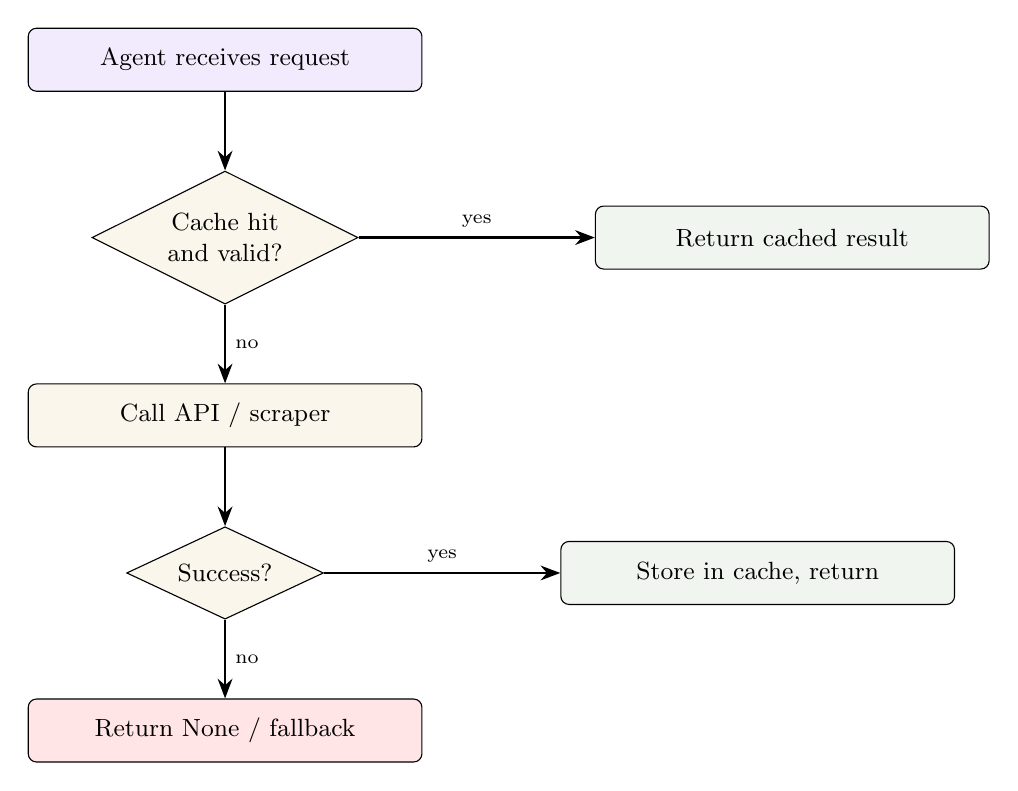
\begin{tikzpicture}[
    node distance=1cm,
    box/.style={draw, rounded corners=3pt, minimum width=5cm, minimum height=0.8cm, font=\small, align=center},
    arr/.style={-{Stealth[length=2.5mm]}, thick},
    decision/.style={draw, diamond, aspect=2, minimum width=2.5cm, font=\small, align=center, fill=gold!10},
]

\node[box, fill=claudepurple!10] (req) {Agent receives request};
\node[decision, below=of req] (check) {Cache hit\\and valid?};
\node[box, fill=nodegreen!10, right=3cm of check] (hit) {Return cached result};
\node[box, fill=gold!10, below=of check] (fetch) {Call API / scraper};
\node[decision, below=of fetch] (ok) {Success?};
\node[box, fill=nodegreen!10, right=3cm of ok] (store) {Store in cache, return};
\node[box, fill=red!10, below=of ok] (fail) {Return None / fallback};

\draw[arr] (req) -- (check);
\draw[arr] (check) -- node[above, font=\scriptsize] {yes} (hit);
\draw[arr] (check) -- node[right, font=\scriptsize] {no} (fetch);
\draw[arr] (fetch) -- (ok);
\draw[arr] (ok) -- node[above, font=\scriptsize] {yes} (store);
\draw[arr] (ok) -- node[right, font=\scriptsize] {no} (fail);

\end{tikzpicture}
\caption{Cache lookup flow for each verification agent.}
\label{fig:cache-flow}
\end{figure}

\begin{techbox}[SQLite Schema]
\begin{lstlisting}[language=SQL]
CREATE TABLE cache (
    key        TEXT PRIMARY KEY,
    value      TEXT NOT NULL,     -- JSON serialized
    created_at REAL NOT NULL,     -- Unix timestamp
    ttl_hours  REAL NOT NULL
);
\end{lstlisting}
A row is valid when \texttt{time() < created\_at + ttl\_hours $\times$ 3600}.
Expired rows are purged on startup and lazily on read.
The entire cache is cleared at the start of each new trip generation.
\end{techbox}


% ══════════════════════════════════════════════════════════════════════════════
\section{Data Flow: End-to-End}
% ══════════════════════════════════════════════════════════════════════════════

\begin{figure}[H]
\centering
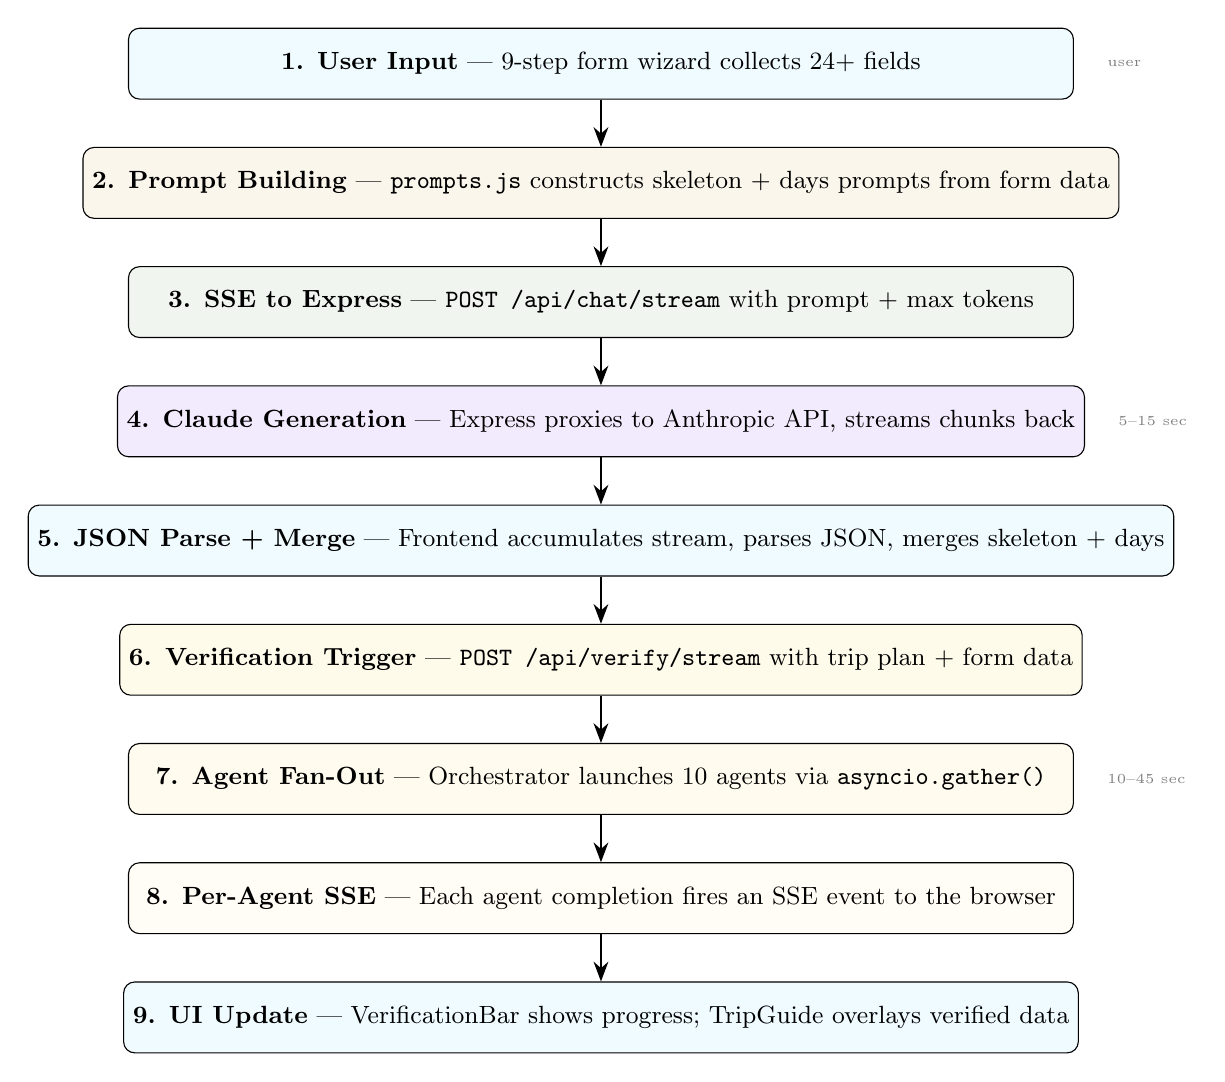
\begin{tikzpicture}[
    node distance=0.6cm,
    phase/.style={draw, rounded corners=4pt, minimum width=12cm, minimum height=0.9cm, font=\small, align=center},
    arr/.style={-{Stealth[length=2.5mm]}, thick},
]

\node[phase, fill=reactblue!10] (p1) {\textbf{1. User Input} --- 9-step form wizard collects 24+ fields};
\node[phase, fill=gold!10, below=of p1] (p2) {\textbf{2. Prompt Building} --- \texttt{prompts.js} constructs skeleton + days prompts from form data};
\node[phase, fill=nodegreen!10, below=of p2] (p3) {\textbf{3. SSE to Express} --- \texttt{POST /api/chat/stream} with prompt + max tokens};
\node[phase, fill=claudepurple!10, below=of p3] (p4) {\textbf{4. Claude Generation} --- Express proxies to Anthropic API, streams chunks back};
\node[phase, fill=reactblue!10, below=of p4] (p5) {\textbf{5. JSON Parse + Merge} --- Frontend accumulates stream, parses JSON, merges skeleton + days};
\node[phase, fill=pythonyellow!10, below=of p5] (p6) {\textbf{6. Verification Trigger} --- \texttt{POST /api/verify/stream} with trip plan + form data};
\node[phase, fill=pythonyellow!8, below=of p6] (p7) {\textbf{7. Agent Fan-Out} --- Orchestrator launches 10 agents via \texttt{asyncio.gather()}};
\node[phase, fill=pythonyellow!5, below=of p7] (p8) {\textbf{8. Per-Agent SSE} --- Each agent completion fires an SSE event to the browser};
\node[phase, fill=reactblue!10, below=of p8] (p9) {\textbf{9. UI Update} --- VerificationBar shows progress; TripGuide overlays verified data};

\foreach \a/\b in {p1/p2, p2/p3, p3/p4, p4/p5, p5/p6, p6/p7, p7/p8, p8/p9} {
    \draw[arr] (\a) -- (\b);
}

% Time annotations
\node[right=0.3cm of p1, font=\tiny\color{gray}] {user};
\node[right=0.3cm of p4, font=\tiny\color{gray}] {5--15 sec};
\node[right=0.3cm of p7, font=\tiny\color{gray}] {10--45 sec};

\end{tikzpicture}
\caption{Complete end-to-end data flow from user input to verified trip display.}
\label{fig:e2e-flow}
\end{figure}


% ══════════════════════════════════════════════════════════════════════════════
\section{SSE Streaming Protocol}
% ══════════════════════════════════════════════════════════════════════════════

Both trip generation and verification use Server-Sent Events (SSE) for real-time streaming.

\subsection{Claude Streaming (Generation)}

\begin{table}[H]
\centering
\begin{tabularx}{\textwidth}{l X}
\toprule
\textbf{Event} & \textbf{Format} \\
\midrule
Text chunk & \texttt{data: \{"text": "partial JSON..."\}} \\
Completion & \texttt{data: [DONE]} \\
Error & \texttt{event: error\textbackslash ndata: \{"error": "message"\}} \\
\bottomrule
\end{tabularx}
\caption{SSE event format for Claude streaming.}
\end{table}

\subsection{Verification Streaming}

\begin{table}[H]
\centering
\begin{tabularx}{\textwidth}{l X}
\toprule
\textbf{Event} & \textbf{Format} \\
\midrule
Agent result & \texttt{data: \{"agent": "weather:Tokyo", "status": \{...\}, "snapshot": \{...\}\}} \\
Completion & \texttt{data: [DONE]} \\
\bottomrule
\end{tabularx}
\caption{SSE event format for verification streaming. Each agent completion fires one event.}
\end{table}

The \texttt{status} object contains: \texttt{agent} (name), \texttt{status} (success/failed), \texttt{duration\_ms}, \texttt{result\_count}, and optionally \texttt{error}.

The \texttt{snapshot} is the cumulative \texttt{VerifyResponse} object with all results received so far.


% ══════════════════════════════════════════════════════════════════════════════
\section{Results Display}
% ══════════════════════════════════════════════════════════════════════════════

The \texttt{TripGuide} component renders the completed trip in a 7-tab layout:

\begin{table}[H]
\centering
\begin{tabularx}{\textwidth}{l X}
\toprule
\textbf{Tab} & \textbf{Content} \\
\midrule
Map & Google Maps embed with route, numbered stops \\
Itinerary & Day-by-day activities with weather, ratings, verification badges \\
Stays & Verified hotel prices + AI accommodation options with booking links \\
Flights & Verified flight prices + AI estimates with search links \\
Budget & Currency conversion, breakdown table, live exchange rates \\
Suggestions & Curated splurges with Maps/booking links \\
Tips & Insider tips, packing list, Instagram accounts, YouTube searches \\
\bottomrule
\end{tabularx}
\caption{The 7 tabs of the TripGuide results view.}
\end{table}

\begin{infobox}[Verification Overlay Strategy]
Every piece of data in the UI displays a verification badge indicating its source:
\begin{itemize}[nosep]
    \item \textcolor{nodegreen}{\textbf{Verified}} (green) --- Confirmed by a verification agent with real data.
    \item \textcolor{claudepurple}{\textbf{AI Estimate}} (purple) --- Generated by Claude, not independently verified.
\end{itemize}
This transparency ensures users know which data points are independently confirmed.
\end{infobox}


% ══════════════════════════════════════════════════════════════════════════════
\section{PDF Export}
% ══════════════════════════════════════════════════════════════════════════════

PDF generation uses \texttt{@react-pdf/renderer} loaded via dynamic \texttt{import()} to keep the initial bundle small (the library is $\sim$1.5\,MB).

\begin{figure}[H]
\centering
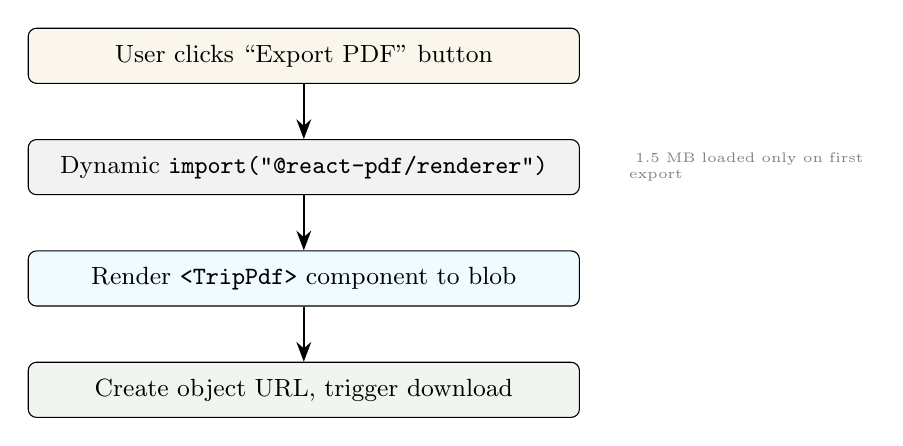
\begin{tikzpicture}[
    node distance=0.7cm,
    box/.style={draw, rounded corners=3pt, minimum width=7cm, minimum height=0.7cm, font=\small, align=center},
    arr/.style={-{Stealth[length=2.5mm]}, thick},
]

\node[box, fill=gold!10] (s1) {User clicks ``Export PDF'' button};
\node[box, fill=gray!10, below=of s1] (s2) {Dynamic \texttt{import("@react-pdf/renderer")}};
\node[box, fill=reactblue!10, below=of s2] (s3) {Render \texttt{<TripPdf>} component to blob};
\node[box, fill=nodegreen!10, below=of s3] (s4) {Create object URL, trigger download};

\foreach \a/\b in {s1/s2, s2/s3, s3/s4} {
    \draw[arr] (\a) -- (\b);
}

\node[right=0.5cm of s2, font=\tiny\color{gray}, text width=3cm] {~1.5 MB loaded only on first export};

\end{tikzpicture}
\caption{Lazy-loaded PDF export flow.}
\label{fig:pdf-export}
\end{figure}

The PDF includes: trip header with stats, travel advisory, day-by-day itinerary, weather forecast, accommodations, budget breakdown, and travel tips.


% ══════════════════════════════════════════════════════════════════════════════
\section{Deployment Architecture}
% ══════════════════════════════════════════════════════════════════════════════

\subsection{Docker Containers}

\begin{figure}[H]
\centering
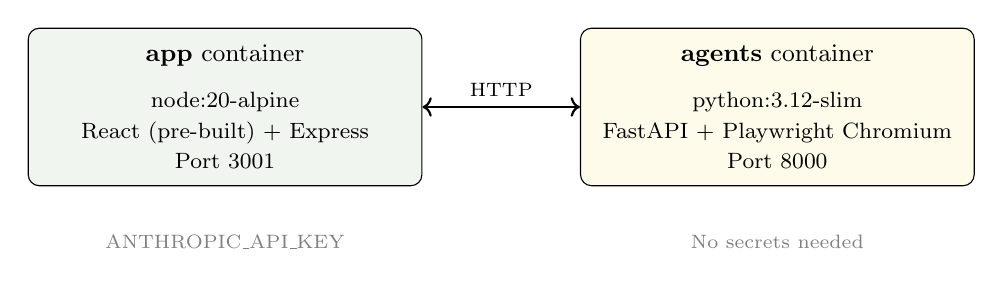
\begin{tikzpicture}[
    node distance=1.5cm,
    container/.style={draw, rounded corners=4pt, minimum width=5cm, minimum height=2cm, font=\small, align=center},
    arr/.style={-{Stealth[length=2.5mm]}, thick},
]

\node[container, fill=nodegreen!10] (app) {
    \textbf{app} container\\[0.2cm]
    {\footnotesize node:20-alpine}\\
    {\footnotesize React (pre-built) + Express}\\
    {\footnotesize Port 3001}
};

\node[container, fill=pythonyellow!10, right=2cm of app] (agents) {
    \textbf{agents} container\\[0.2cm]
    {\footnotesize python:3.12-slim}\\
    {\footnotesize FastAPI + Playwright Chromium}\\
    {\footnotesize Port 8000}
};

\draw[arr, <->] (app) -- node[above, font=\scriptsize] {HTTP} (agents);

\node[below=0.5cm of app, font=\scriptsize\color{gray}] {ANTHROPIC\_API\_KEY};
\node[below=0.5cm of agents, font=\scriptsize\color{gray}] {No secrets needed};

\end{tikzpicture}
\caption{Docker Compose deployment with two containers.}
\label{fig:docker}
\end{figure}

The \texttt{app} container uses a multi-stage Dockerfile:
\begin{enumerate}[nosep]
    \item \textbf{Stage 1:} \texttt{node:20-alpine} builds the React frontend (\texttt{npm run build}).
    \item \textbf{Stage 2:} \texttt{node:20-alpine} with production dependencies only, copies built \texttt{dist/} from Stage 1, runs \texttt{node server.js}.
\end{enumerate}

The \texttt{agents} container installs system dependencies for Playwright, then installs Chromium and Python dependencies.

\subsection{Supported Platforms}

\begin{table}[H]
\centering
\begin{tabularx}{\textwidth}{l X}
\toprule
\textbf{Platform} & \textbf{Configuration} \\
\midrule
Docker Compose & Two services, local development or self-hosted \\
Railway & Two services linked via internal networking \\
Render & Two Web Services (Node + Python) \\
Fly.io & Two apps with internal DNS (\texttt{.internal:8000}) \\
AWS ECS / Cloud Run / Azure & Container deployment from Docker Hub images \\
\bottomrule
\end{tabularx}
\caption{Supported deployment platforms.}
\end{table}


% ══════════════════════════════════════════════════════════════════════════════
\section{Security and Error Handling}
% ══════════════════════════════════════════════════════════════════════════════

\begin{itemize}[nosep]
    \item \textbf{API key validation:} The server validates the Anthropic key format on startup and rejects placeholder values.
    \item \textbf{Rate limiting:} Three tiers of rate limiting protect the Claude API and verification service.
    \item \textbf{Request size limit:} JSON body parsing capped at 1\,MB.
    \item \textbf{Timeout guards:} 60-second timeout on non-streaming verify, 120-second on streaming, 45-second per-agent timeout.
    \item \textbf{CORS:} Open CORS for development; should be restricted in production.
    \item \textbf{No secrets in frontend:} The API key never leaves the server; the browser only talks to Express.
    \item \textbf{Graceful degradation:} If the Python service is down, the app works fully with AI estimates.
    \item \textbf{Scraper resilience:} Anti-bot 403s are expected and handled via fallback chains.
\end{itemize}


% ══════════════════════════════════════════════════════════════════════════════
\section{Parameter Flow}
% ══════════════════════════════════════════════════════════════════════════════

User form inputs flow to two destinations: the Claude prompts (for AI personalization) and the verification agents (for data lookup).

\begin{figure}[H]
\centering
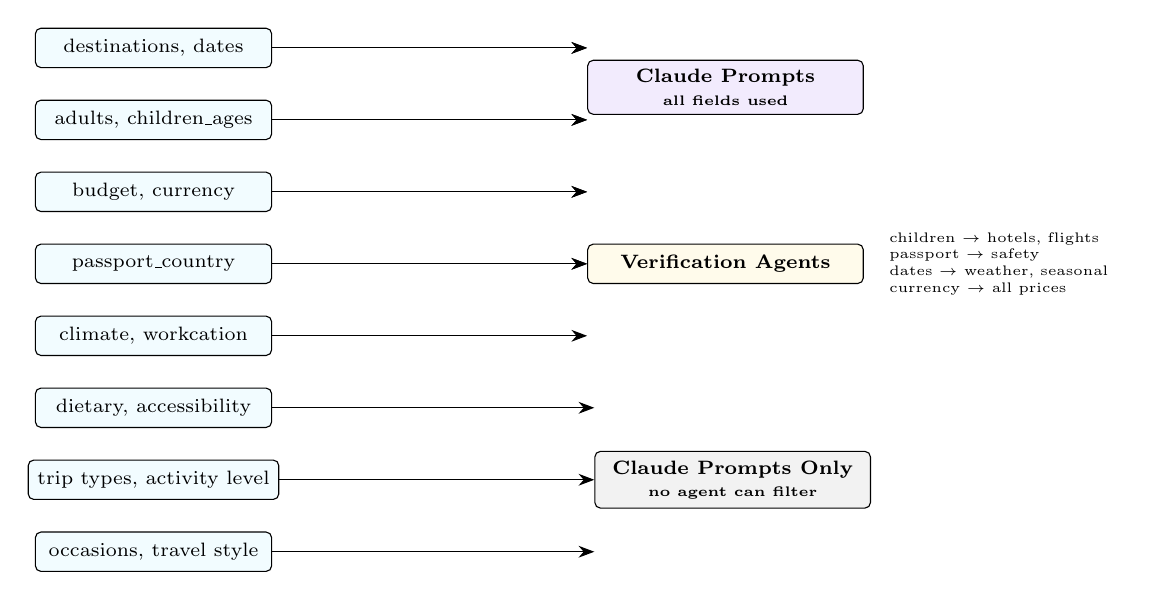
\begin{tikzpicture}[
    node distance=0.4cm,
    field/.style={draw, rounded corners=2pt, minimum width=3cm, minimum height=0.5cm, font=\scriptsize, align=center, fill=reactblue!8},
    target/.style={draw, rounded corners=2pt, minimum width=3.5cm, minimum height=0.5cm, font=\scriptsize\bfseries, align=center},
    arr/.style={-{Stealth[length=2mm]}},
]

% Form fields - left
\node[field] (f1) {destinations, dates};
\node[field, below=of f1] (f2) {adults, children\_ages};
\node[field, below=of f2] (f3) {budget, currency};
\node[field, below=of f3] (f4) {passport\_country};
\node[field, below=of f4] (f5) {climate, workcation};
\node[field, below=of f5] (f6) {dietary, accessibility};
\node[field, below=of f6] (f7) {trip types, activity level};
\node[field, below=of f7] (f8) {occasions, travel style};

% Targets - right
\node[target, fill=claudepurple!10, right=4cm of f1, yshift=-0.5cm] (claude) {Claude Prompts\\{\tiny all fields used}};
\node[target, fill=pythonyellow!10, right=4cm of f4] (agents) {Verification Agents};
\node[target, fill=gray!10, right=4cm of f7] (prompt) {Claude Prompts Only\\{\tiny no agent can filter}};

% Arrows to both
\foreach \f in {f1, f2, f3} {
    \draw[arr] (\f.east) -- (claude.west |- \f);
    \draw[arr, dashed] (\f.east) -- (agents.west |- \f);
}
\draw[arr] (f4.east) -- (claude.west |- f4);
\draw[arr, dashed] (f4.east) -- (agents.west |- f4);
\draw[arr] (f5.east) -- (claude.west |- f5);

% Arrows to Claude only
\foreach \f in {f6, f7, f8} {
    \draw[arr] (\f.east) -- (prompt.west |- \f);
}

% Annotations
\node[right=0.2cm of agents, font=\tiny, text width=3cm, align=left] {
    children $\to$ hotels, flights\\
    passport $\to$ safety\\
    dates $\to$ weather, seasonal\\
    currency $\to$ all prices
};

\end{tikzpicture}
\caption{Parameter flow from form fields to Claude prompts and verification agents.}
\label{fig:param-flow}
\end{figure}


% ══════════════════════════════════════════════════════════════════════════════
\section{Pydantic Data Models}
% ══════════════════════════════════════════════════════════════════════════════

The Python verification service uses Pydantic models for all request/response schemas.

\begin{table}[H]
\centering
\small
\begin{tabularx}{\textwidth}{l X}
\toprule
\textbf{Model} & \textbf{Key Fields} \\
\midrule
\texttt{VerifyRequest} & \texttt{trip\_plan}, destinations, dates, adults, children\_ages, passport\_country, currency, budget \\
\texttt{VerifyResponse} & \texttt{weather\{\}}, \texttt{safety\{\}}, \texttt{seasonal\{\}}, \texttt{currency}, \texttt{places[]}, \texttt{hotels\{\}}, \texttt{activities[]}, \texttt{reviews[]}, \texttt{flights[]}, \texttt{links[]}, \texttt{agent\_statuses[]}, \texttt{verification\_score} \\
\texttt{AgentStatus} & agent name, status (success/failed), duration\_ms, result\_count, error \\
\texttt{WeatherDay} & date, temp\_high, temp\_low, precipitation, weather\_code, icon \\
\texttt{SafetyResult} & score (0--5), level, emoji, alerts[], advice \\
\texttt{HotelResult} & name, price\_per\_night, rating, review\_count, source, booking\_url \\
\texttt{FlightResult} & airline, price, duration, stops, source, booking\_url \\
\texttt{PlaceVerification} & found (bool), lat, lon, address, confidence, maps\_url \\
\texttt{ReviewResult} & place\_name, rating (1--5), review\_count, snippets[] \\
\bottomrule
\end{tabularx}
\caption{Key Pydantic models and their fields.}
\end{table}


% ══════════════════════════════════════════════════════════════════════════════
\section{Configuration}
% ══════════════════════════════════════════════════════════════════════════════

Agent behavior is controlled by \texttt{agents/config.py}:

\begin{itemize}[nosep]
    \item Each agent has an \texttt{enabled} flag that can be toggled off.
    \item Optional API keys (\texttt{SERPAPI\_KEY}, \texttt{AMADEUS\_KEY}, \texttt{VIATOR\_API\_KEY}, \texttt{GOOGLE\_PLACES\_KEY}) auto-upgrade agents from scraping to paid API providers when set.
    \item Scraping parameters: viewport size ($1920 \times 1080$), delay range (1--3 seconds), 6 user agents for rotation.
\end{itemize}


% ══════════════════════════════════════════════════════════════════════════════
\section{Cost Analysis}
% ══════════════════════════════════════════════════════════════════════════════

\begin{table}[H]
\centering
\begin{tabularx}{\textwidth}{l c X}
\toprule
\textbf{Component} & \textbf{Cost} & \textbf{Notes} \\
\midrule
All 10 verification agents & \$0 & Free APIs + web scraping \\
Claude API (per trip) & \$0.01--0.05 & Two API calls: skeleton + days \\
Hosting (Docker) & Variable & Depends on platform \\
\bottomrule
\end{tabularx}
\caption{Cost breakdown per trip generation.}
\end{table}


% ══════════════════════════════════════════════════════════════════════════════
\section*{Appendix: File Map}
% ══════════════════════════════════════════════════════════════════════════════

\begin{table}[H]
\centering
\small
\begin{tabularx}{\textwidth}{l X}
\toprule
\textbf{File} & \textbf{Responsibility} \\
\midrule
\multicolumn{2}{l}{\textit{Frontend}} \\
\texttt{src/main.jsx} & React entry point \\
\texttt{src/App.jsx} & App shell, view routing \\
\texttt{src/context/TripContext.jsx} & All state, generation logic \\
\texttt{src/prompts.js} & Claude prompt construction \\
\texttt{src/api.js} & HTTP client, SSE reader, JSON parser \\
\texttt{src/hooks/useVerification.js} & Verification SSE hook \\
\texttt{src/components/FormSteps.jsx} & 9-step wizard \\
\texttt{src/components/TripGuide.jsx} & 7-tab results display \\
\texttt{src/components/PdfExport.jsx} & Lazy PDF generation \\
\midrule
\multicolumn{2}{l}{\textit{Backend}} \\
\texttt{server.js} & Express gateway, SSE proxy \\
\midrule
\multicolumn{2}{l}{\textit{Python Verification}} \\
\texttt{agents/main.py} & FastAPI app, SSE endpoint \\
\texttt{agents/orchestrator.py} & Parallel agent dispatch \\
\texttt{agents/models.py} & Pydantic schemas \\
\texttt{agents/config.py} & Agent toggles, scraping config \\
\texttt{agents/cache.py} & SQLite TTL cache \\
\texttt{agents/agents/*.py} & 10 agent wrappers \\
\texttt{agents/scrapers/*.py} & Playwright + httpx scrapers \\
\texttt{agents/free\_apis/*.py} & Free API integrations \\
\bottomrule
\end{tabularx}
\caption{Complete file map with responsibilities.}
\end{table}

\end{document}
